

\section{Úkol 1}

Jednotlivé politické strany \( \left\{ a_1, \dots, a_{25} \right \} \), kde \( a_i \in \bbR^{100} \) je možné chápat jako body v prostoru odpovědí na referenční programové otázky. Chtěli bychom tento prostor vhodně vizualizovat. To uděláme tak, že body \( a_i \) proložíme \bf{afinním} podprostorem dimenze 2, tak aby součet kvadrátů vzdáleností původních \( a_i \) a promítnutých bodů \( a'_i \) byl minimální. Následně promítnuté body zobrazíme v souřadnicích báze nalezeného afinního podprostoru.

\begin{enumerate}
    \item Formulujte optimalizační problém.

    Hledáme bázi afinního podprostoru dimenze 2, jehož body \( a'_i \) mají od bodů \( a_i \) nej\-menší vzdálenost. Pro body \( a'_i \) a \( a_i \) tedy platí, že
    \[ \min \lVert a'_i - a_i \rVert, i \in \left[ 1, 25 \right]. \]

    \item Vyřešte optimalizační problém.

    Prostor, ve kterém se nacházejí body \( a_i, i \in \left[ 1, 25 \right] \) posuneme pomocí těžiště těchto bodů do počátku a spektrálním rozkladem získáme matici vlastních vektorů \( V \) a matici vlastních čísel \( D \). S využitím věty 7.3 získáme bázi hledáného podprostoru tak, že vezmeme poslední 2 sloupce matice \( V \) (tj. dva vlastní vektory příslušející dvěma největším vlastním číslům). Tyto vektory tvoří ortonormální bázi hledáného podprostoru.

    Kritériem je nazvána hodnota stopy matice \( A \), což je součet \( k \) nejmenších vlastních čísel matice \( A \). S využitím věty 7.2 získáme vzorec
    \[ \min \left\{ \mathrm{tr} \lr{X^T A X} \| X \in \bbR^{n \times k}, X^T X = \bf{I} \right\} = \lambda_1 + \cdots + \lambda_k \]

    S využitím Matlabu
    \begin{lstlisting}[style=Matlab-editor]
sum(sum(D(1:end - 2,:)))
    \end{lstlisting}

    získáváme \( \mathrm{tr} \lr{A} = 1 098,1 \).

    \item Najděte ortonormální bázi nalezeného afinního podprostoru \( \mathrm{span} \left\{ a'_1, \dots, a'_{25} \right \} + a_0 \) a jednotlivé politické strany zobrazte v souřadnicích této báze (jejíž vektory ztotožníte s osami 2D grafu). Zakreslené body obarvěte barvou strany (podle \verb|T.color|).

    \begin{center}
        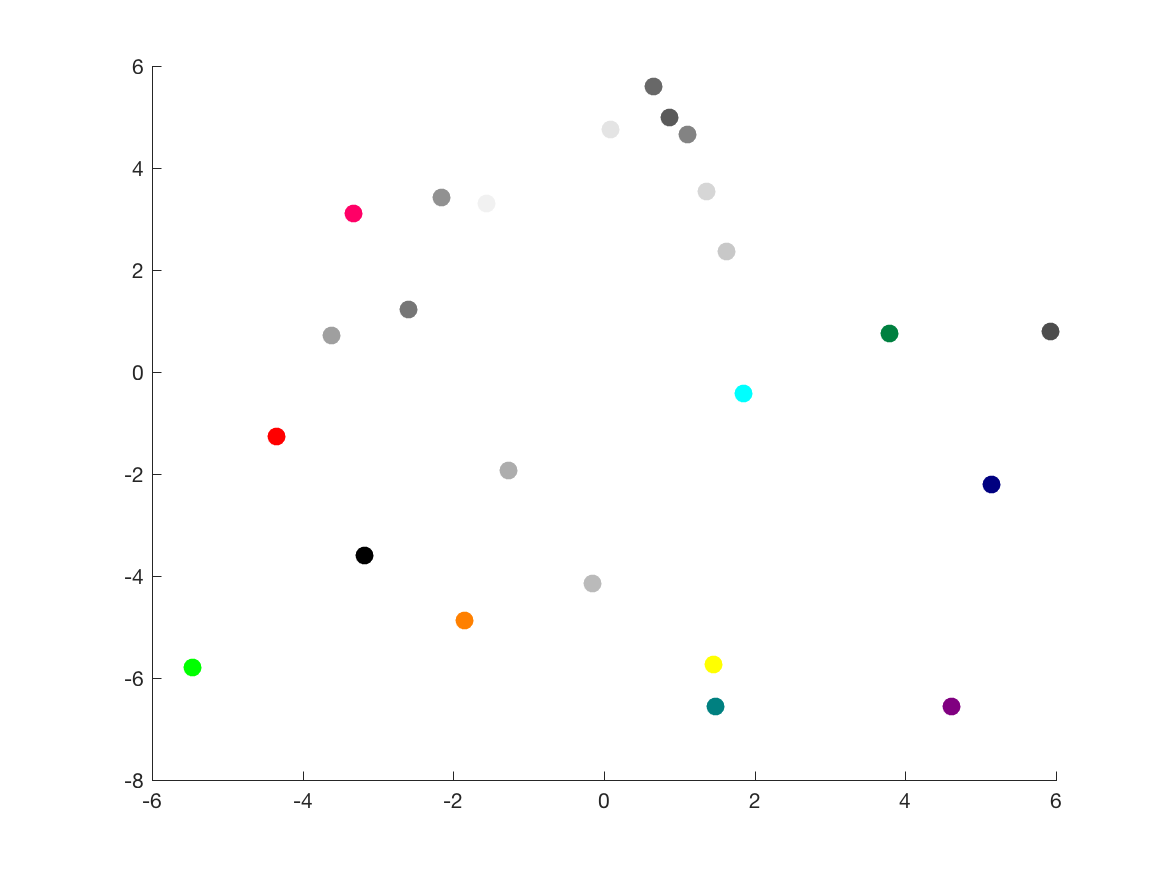
\includegraphics[width=\textwidth]{../strany.png}
    \end{center}

    \item Interpretujte výsledek.

    Dle výsledného grafu se strany podle svislé osy pravděpodobně rozdělily na pravicové a levicové. Rozdělení podle vodorovné osy není zřejmé.

\end{enumerate}

\newpage

\section{Úkol 2}

Vizualizovat tato data je možné i z opačného pohledu. Jednotlivé otázky \( \left\{ b_1, \dots, b_{100} \right\} \), kde \( b_i \in \bbR^{25} \) jsou body v prostoru politických stran. Otázky zobrazíme opět v prostoru dimenze 2.

\begin{enumerate}
    \item Postupujte obdobně jako v minulém příkladu a zakreselete jednotlivé otázky v sou\-řadnicích ortonormální báze dimenze 2 prostoru proložení ve smyslu nejmenších čtverců. Výsledné body obarvěte podle toho, zda většina politických stran odpovídá ano.

    \begin{center}
        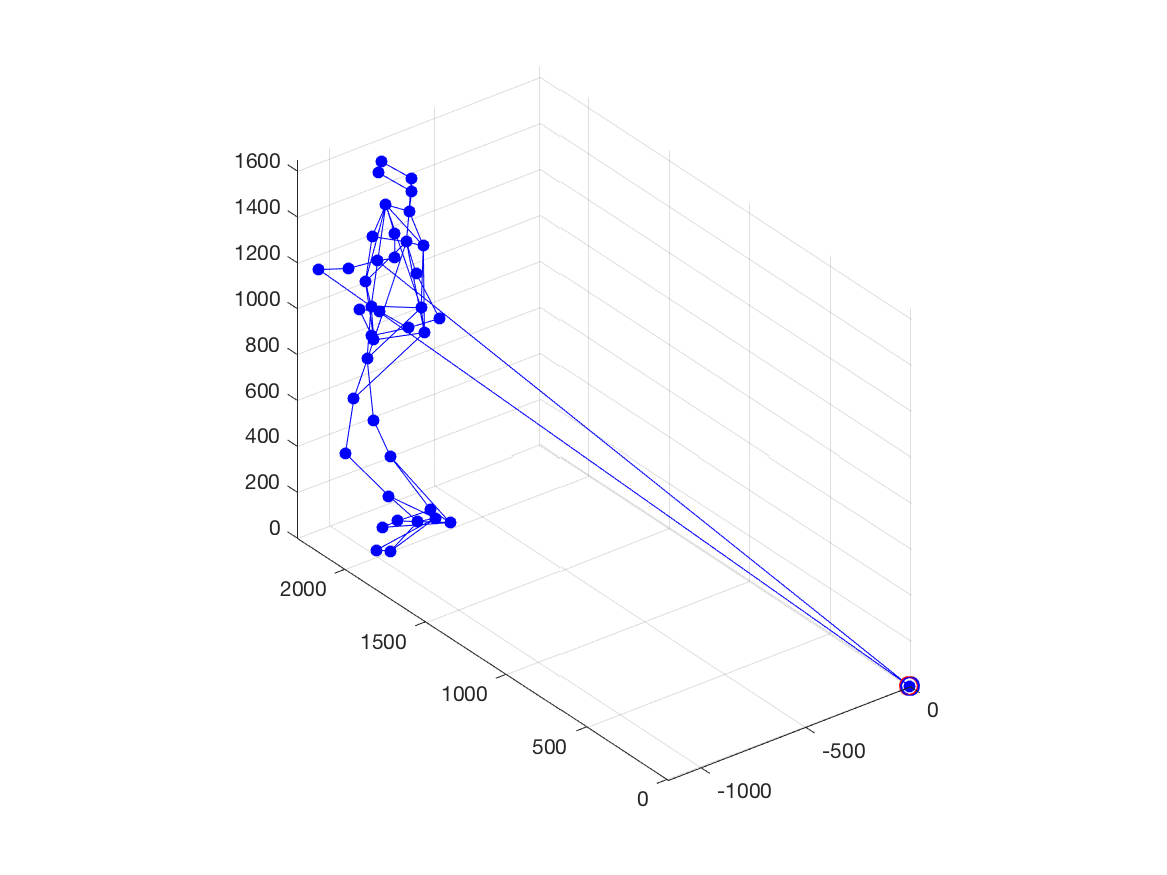
\includegraphics[width=\textwidth]{../otazky.png}
    \end{center}

    \item Interpretujte výsledek.

    Vizualizací otázek do podprostoru dimenze 2 došlo ke grafickému oddělení jednotlivých otázek podle toho, jestli na ně strany častěji odpovídaly ano či ne. Červeně obarvené jsou ty otázky, na které většina politických stran odpovídala ano a modře jsou otázky s většinovým podílem záporných odpovědí.

    \item Je možné nalézt ortonormální bázi hledaného podprostoru a souřadnice promítnutých bodů v této bázi využitím výpočtu z předchozího úkolu? Pokud ano, vysvětlete.

    V druhém úkolu se pracuje se stejnou vstupní matici, avšak tato matice je transponovaná. Pro řešení tohoto úkolu lze využít stejný postup jako v případě Úkol č. 1 s menšími úpravami, ale finální výsledky se rozhodně liší.

\end{enumerate}

\newpage

\section{Příloha}

\subsection{Zdrojový kód pro řešení úkolu č. 1}

\lstinputlisting[style=Matlab-editor]{../ukol_1.m}

\subsection{Zdrojový kód pro řešení úkolu č. 2}

\lstinputlisting[style=Matlab-editor]{../ukol_2.m}
